\section{Identidad}

Todo este tiempo hemos trabajado con la tabla "Personas", esta posee la columna "id", esta columna es un identificador para cada registro en nuestra tabla, un identificador que diferencia un registro de otro. Esta columna suele ser del tipo entero (INT), no permite valores NULL y se llama "id", "Id" o "ID", el comando \textbf{AUTO\_INCREMENT} permite que con cada nuevo registro insertado, el valor de la columna "id" auto incremente: si tenemos tres registro e insertamos uno nuevo, el id del nuevo registro será cuatro automáticamente.

Esta columna es muy importante en todas las tablas, porque el el índice que nos permite seleccionar registros de forma rápida sin tener que utilizar el resto de columnas (nombre, apellidos, ciudad y edad en este caso). Un ejemplo de como configurar esta columna "id" es el siguiente:
\begin{lstlisting}
    CREATE TABLE Pilotos(
        id INT NOT NULL AUTO_INCREMENT,
        nombres varchar(50),
        apellidos varchar(50)
    );
\end{lstlisting}

De esta manera, cada nuevo registro tendrá un id automático auto incrementable y no deberemos especificarlo en la inserción:
\begin{lstlisting}
    INSERT INTO Pilotos(nombre, apellidos)
    VALUES
        ('pancho', 'villa'),
        ('emiliano', 'zapata'),
        ('porfirio', 'diaz');
\end{lstlisting}

Esta tabla "Pilotos" queda como en la \textit{Tabla \ref{tab: 31}}:
\begin{table}[H]
    \centering
    \caption{Registros con id auto incrementable}
    \label{tab: 31}
    \begin{tabular}{|l|l|l|}
        \hline
        \textbf{id} & \textbf{nombres} & \textbf{apellidos} \\
        \hline
        1 & pancho      & villa \\
        \hline
        2 & emiliano    & zapata \\
        \hline
        3 & porfirio    & diaz \\
        \hline
    \end{tabular}
\end{table}

El comando \textit{AUTO\_INCREMENT} tiene como valor de inicio el 1, se puede cambiar al momento de la creación de la tabla o ya creada:
\begin{lstlisting}
    -- Creando la tabla.
    CREATE TABLE demo(
        id INT NOT NULL AUTO_INCREMENT = 100, ...
    )

    -- Modificando la tabla "Pilotos".
    ALTER TABLE Pilotos
        AUTO_INCREMENT=200
\end{lstlisting}

Si la tabla fue creada previamente y se modifica el valor inicial de AUTO\_INCREMENT, los siguientes registros a esta modificación ya serán con el nuevo valor inicial, los registros anteriores se mantendrán con el valor con el que fueron insertados.



\section{Llaves Primarias y Secundarias}

La \textbf{llave primaria} (\textbf{PRIMARY KEY}) de una tabla es una columna que permite la relación con otras tablas, por ejemplo: una sola persona puede tener múltiples números de celular, sería problemático tener varios registros de una persona con distinto número de celular, por lo que sería recomendable crear una tabla aparte con únicamente números de celular de cada persona; debemos hacer que tengan una relación las personas (tabla "Personas") con los números que poseen (nueva tabla "NumCel"), por lo que debemos establecer una llave primaria en alguna de las tablas para iniciar esa relación, ahí entra la columna "id", la cual generalmente es la llave primaria gracias a las siguientes características o reglas:
\begin{itemize}
    \item Debe contener valores \textbf{únicos}.
    \item No debe tener valores \textbf{NULL}.
    \item Una tabla debe tener \textbf{solamente una} llave primaria.
\end{itemize}

Repetiremos la creación de la tabla "Personas" pero con la asignación de la llave primaria a la columna "id" y crearemos la tabla "NumCel" para ejemplificar esta lección:
\begin{lstlisting}
    CREATE TABLE Personas(
        id INT NOT NULL AUTO_INCREMENT,
        nombre VARCHAR(255),
        apellidos VARCHAR(255),
        ciudad (VARCHAR255)
        edad INT,
        PRIMARY KEY (id)
    );

    CREATE TABLE PhoneNumbers (
        id INT NOT NULL AUTO_INCREMENT,
        id_persona INT NOT NULL,
        numero VARCHAR(55),
        tipo VARCHAR(55),
        PRIMARY KEY (id),
        FOREIGN KEY (customer_id) REFERENCES Personas(id)
    );
\end{lstlisting}

El comando \textbf{PRIMARY KEY ()} permite asignar la llave primaria de una tabla a una columna. Ahora la tabla "Personas" tiene como llave primaria a la columna "id", mientras que la tabla "NumCel" tiene a "id" como llave primaria. Hasta este punto, todavía no hay relación entre ambas tablas, debemos mencionar lo que es una llave foránea.

Una \textbf{llave foránea} (\textbf{FOREIGN KEY}) es una columna que crea la relación entre las tablas, en una tabla Y se crea una columna con los valores de una tabla X para cada registro de la tabla Y que tengan relación. Veamos el ejemplo anterior de una manera más visual en la \textit{Figura \ref{fig: 1}}:
\begin{figure}[H]
    \centering
    \caption{Relación entre dos tablas}
    \label{fig: 1}
    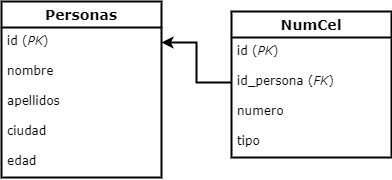
\includegraphics[width=8cm]{ss/relacion_tablas.jpg}
\end{figure}

Ambas tablas tienen su llave primaria junto con sus registros, pero la tabla "NumCel" tiene una columna llamada "id\_persona" que contiene los ids de las personas de la columna "id" de la tabla "Personas", por lo que esta columna es la que realmente hace la relación entre ambas columnas; la llave foránea de una tabla es la que conecta con la llave primaria de la otra tabla.

El comando \textbf{FOREIGN KEY ()} permite asignar la llave foránea de una tabla a una columna, analicemos el siguiente comando:
\begin{lstlisting}
    FOREIGN KEY (customer_id) REFERENCES Personas(id)
\end{lstlisting}

\textit{FOREIGN KEY (customer\_id)} asigna la llave foránea a la columna "customer\_id" de la tabla "NumCel", y \textit{REFERENCES Personas(id)} es la llave primaria de la tabla a relacionar, es aquí donde se crea la relación (en código) de ambas tablas. Insertamos algunos registros en la tabla "NumCel" y veamos visualmente como se ve el resultado en la \textit{Figura \ref{fig: 2}}:
\begin{figure}[H]
    \centering
    \caption{Tablas relacionadas}
    \label{fig: 2}
    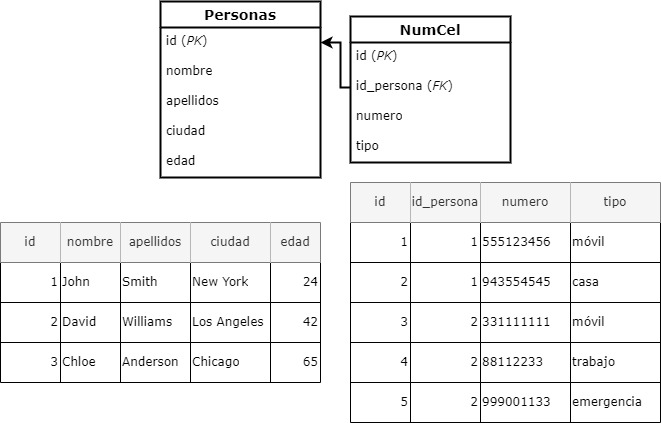
\includegraphics[width=11cm]{ss/tablas_relacionadas.jpg}
\end{figure}

\textit{Nota}: una tabla puede tener múltiples llaves foráneas.



\section{Llaves Únicas}

Las \textbf{llaves únicas} (\textbf{UNIQUE}) son columnas que poseen valores únicos (no duplicados) pero no son el identificador ni llave primaria de la tabla, una tabla puede tener varias llaves únicas, pero una sola llave primaria. Haremos que la columna "apellidos" de la tabla "Personas" sea una llave única:
\begin{lstlisting}
    ALTER TABLE Personas
    ADD UNIQUE apellidos
\end{lstlisting}

Ahora, cada apellido de cada registro no podrá estar duplicado, por lo que si intentamos insertar un registro con el apellido "Anderson" u alguno otro de esta tabla tendremos un error. Los valores \textit{NULL} son ignorados en una llave única, por lo que podemos tener múltiples valores NULL en estas columnas.
